\documentclass[12pt,twoside]{report}
\setcounter{secnumdepth}{3}

\usepackage[utf8]{inputenc}
\usepackage{hyperref}
\usepackage{graphicx}
\usepackage[a4paper,width=150mm,top=25mm,bottom=25mm,bindingoffset=6mm]{geometry}
%\usepackage{fancyhdr}
\usepackage[pagestyles]{titlesec}
\usepackage{lipsum}
\usepackage{tikz}
\usepackage{float}
\usepackage{booktabs}
\usepackage{csquotes}
\usepackage{amsmath}
\usepackage{amsthm}
\usepackage{enumitem}
\usepackage{datetime}
\usepackage{subcaption}
\usepackage[titletoc]{appendix}
\usepackage{titlesec}

\usetikzlibrary{shapes,arrows,trees,positioning}
\tikzstyle{block}=[draw, fill=blue!20, minimum size=2em]

\hypersetup{
    colorlinks=true,
    linkcolor=blue,
    filecolor=magenta,      
    urlcolor=blue,
    citecolor=blue
}

%\pagestyle{fancy}
%\renewcommand{\chaptermark}[1]{\markboth{#1}{#1}}
%\fancyhead{}
%\fancyhead[L]{Chapter \thechapter: \leftmark}
%\fancyhead[R]{\nouppercase{\rightmark}}

\renewcommand*\thesection{\arabic{section}}
\newpagestyle{Headings}{
 \sethead
   {Chapter \thechapter: \chaptertitle}
   {}
   {Section \toptitlemarks\thesection: \toptitlemarks\sectiontitle}
   \headrule
 \setfoot{}{\thepage}{}
}
\newpagestyle{PageNum}{
 \setfoot{}{\thepage}{}
}

\theoremstyle{definition}
\newtheorem{definition}{Definition}
\newtheorem{challenge}{Challenge}

\newcommand{\tabitem}{~~\llap{\textbullet}~~}

\graphicspath{ {media/} }

\newcommand{\reporttitle}{Using Answer Set Grammars For Text Summarization}
\newcommand{\reportauthor}{Julien Amblard}
\newcommand{\supervisor}{Alessandra Russo}
\newcommand{\helper}{David Tuckey}
\newcommand{\secondmarker}{Krysia Broda}
\newcommand{\asgauthor}{Mark Law}
\newcommand{\reporttype}{Individual Project}
\newcommand{\degreetype}{Computing MEng}

\begin{document}

\pagestyle{empty}
% Last modification: 2015-08-17 (Marc Deisenroth)
\begin{title}

\newcommand{\HRule}{\rule{\linewidth}{0.5mm}} % Defines a new command for the horizontal lines, change thickness here

%----------------------------------------------------------------------------------------
%	LOGO SECTION
%----------------------------------------------------------------------------------------


\includegraphics[width = 4cm]{imperial_logo.eps}\\[0.5cm] 

\center % Center everything on the page
 
%----------------------------------------------------------------------------------------
%	HEADING SECTIONS
%----------------------------------------------------------------------------------------

\textsc{\LARGE \reporttype}\\[1.5cm] 
\textsc{\Large Department of Computing}\\[0.5cm] 
\textsc{\large Imperial College of Science, Technology and Medicine}\\[0.5cm] 

%----------------------------------------------------------------------------------------
%	TITLE SECTION
%----------------------------------------------------------------------------------------

\HRule \\[0.4cm]
{ \huge \bfseries \reporttitle}\\ % Title of your document
\HRule \\[1.5cm]
 
%----------------------------------------------------------------------------------------
%	AUTHOR SECTION
%----------------------------------------------------------------------------------------

\begin{minipage}{0.4\textwidth}
\begin{flushleft} \large
\emph{Author:}\\
\reportauthor % Your name
\end{flushleft}
\end{minipage}
~
\begin{minipage}{0.4\textwidth}
\begin{flushright} \large
\emph{Supervisor:} \\
\supervisor % Supervisor's Name
\end{flushright}
\end{minipage}\\[4cm]




%----------------------------------------------------------------------------------------


%----------------------------------------------------------------------------------------
%	DATE SECTION
%----------------------------------------------------------------------------------------

{\large \today} % Date, change the \today to a set date if you want to be precise


\vfill % Fill the rest of the page with whitespace
Submitted in partial fulfillment of the requirements for the \degreetype~of Imperial College London

\end{title}


\pagenumbering{roman}

\tableofcontents

\titleformat{\chapter}
{\normalfont\huge}{\chaptertitlename{} \thechapter}{20pt}{\bfseries\huge}
\titlespacing*{\chapter}{0pt}{0pt}{40pt}

\chapter{Introduction}
\pagestyle{Headings}
\pagenumbering{arabic}

- General Problem

- Specific Problem

- Objectives

\chapter{Background}

- Learning answer sets -> learning ASG

- Encoder-decoder overview

\chapter{Contributions}
\begin{figure}[H]
\centering
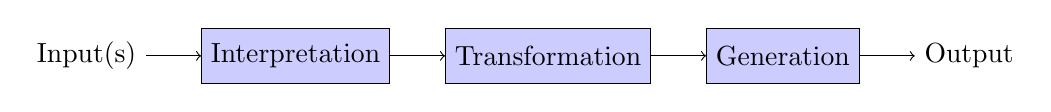
\begin{tikzpicture}[node distance=0.7cm, auto]
\node (input) [] {Input(s)};
\node (interpretation) [block, right =of input] {Interpretation};
\node (transformation) [block, right =of interpretation] {Transformation};
\node (generation) [block, right =of transformation] {Generation};
\node (output) [right =of generation] {Output};
\draw [->] (input) -- (interpretation);
\draw [->] (interpretation) -- (transformation);
\draw [->] (transformation) -- (generation);
\draw [->] (generation) -- (output);
\end{tikzpicture}
\caption{\cite{lloret_text_2008} Summarization Steps}
\label{fig:summarization_steps}
\end{figure}

- Overview of architecture

- Lots of interesting examples

\chapter{Preprocessor}

- Sub diagrams

- Motivate steps (Preprocessor make job easier for ASG, making better quality summary)

\chapter{ASG}
\chapter{ASG}

\textcolor{red}{\textbf{\hl{TODO fix margin, separate task1 from task2 code}}}

\begin{lstlisting}
start -> s_group {
   :- count(X)@1, X > 1.
   :- count(X)@1, X = 0.
}

s_group -> {
  count(0).
}

s_group -> s_group s ". " {
  count(X+1) :- count(X)@1.

  % Reject output summaries with duplicate sentences
  sentence(X,V,O,S) :- output(_,V,O,S)@2, count(X).
  sentence(X,V,O,S) :- sentence(X,V,O,S)@1.
  :- sentence(X1,V,O,S), sentence(X2,V,O,S), X1 != X2.
}

s -> np vp {
  :- not action(verb(V_N,V_T),subject(S_N,S_D,S_A),object(O_N,O_D,O_A)), verb(V_N,V_T)@2, subject(S_N,S_D,S_A)@1, object(O_N,O_D,O_A)@2.

  subject :- subject(S_N,S_D,S_A)@1.
  :- not subject.
  object :- object(S_N,S_D,S_A)@2.
  :- not object.
}

vp -> vbn np {
  verb(N,T) :- verb(N,T)@1.
  object(N,D,A) :- object(N,D,A)@2.
}

vp -> vbd np {
  verb(N,T) :- verb(N,T)@1.
  object(N,D,A) :- object(N,D,A)@2.
}

vp -> vbd vbg np {
  verb(comp(N1,N2),comp(T1,gerund)) :- verb(N1,T1)@1, verb(N2,gerund)@2.
  object(N,D,A) :- object(N,D,A)@3.
}

vp -> vbd vbn np {
  verb(comp(N1,N2),comp(T1,past_part)) :- verb(N1,T1)@1, verb(N2,past_part)@2.
  object(N,D,A) :- object(N,D,A)@3.
}

vp -> vbd "to " vb np {
  verb(comp(N1,N2),comp(T1,base)) :- verb(N1,T1)@1, verb(N2,base)@3.
  object(N,D,A) :- object(N,D,A)@4.
}

vp -> vbp np {
  verb(N,T) :- verb(N,T)@1.
  object(N,D,A) :- object(N,D,A)@2.
}

vp -> vbp vbg np {
  verb(comp(N1,N2),comp(T1,gerund)) :- verb(N1,T1)@1, verb(N2,gerund)@2.
  object(N,D,A) :- object(N,D,A)@3.
}

vp -> vbp vbn np {
  verb(comp(N1,N2),comp(T1,past_part)) :- verb(N1,T1)@1, verb(N2,past_part)@2.
  object(N,D,A) :- object(N,D,A)@3.
}

vp -> vbp "to " vb np {
  verb(comp(N1,N2),comp(T1,base)) :- verb(N1,T1)@1, verb(N2,base)@3.
  object(N,D,A) :- object(N,D,A)@4.
}

vp -> vbz np {
  verb(N,T) :- verb(N,T)@1.
  object(N,D,A) :- object(N,D,A)@2.
}

vp -> vbz vbg np {
  verb(comp(N1,N2),comp(T1,gerund)) :- verb(N1,T1)@1, verb(N2,gerund)@2.
  object(N,D,A) :- object(N,D,A)@3.
}

vp -> vbz vbn np {
  verb(comp(N1,N2),comp(T1,past_part)) :- verb(N1,T1)@1, verb(N2,past_part)@2.
  object(N,D,A) :- object(N,D,A)@3.
}

vp -> vbz "to " vb np {
  verb(comp(N1,N2),comp(T1,base)) :- verb(N1,T1)@1, verb(N2,base)@3.
  object(N,D,A) :- object(N,D,A)@4.
}

np -> np rb {
  object(N,D,A) :- object(N,D,0)@1, adj_or_adv(A)@2.
}

np -> np rb {
  object(N,D,conjunct(A1,A2)) :- object(N,D,A1)@1, adj_or_adv(A2)@2.
  :- object(N,D,conjunct(A,A)).
}

np -> np rp {
  object(N,D,A) :- object(N,D,0)@1, adj_or_adv(A)@2.
}

np -> np rp {
  object(N,D,conjunct(A1,A2)) :- object(N,D,A1)@1, adj_or_adv(A2)@2.
  :- object(N,D,conjunct(A,A)).
}

np -> nn {
  subject(N,0,0) :- noun(N)@1.
  object(N,0,0) :- noun(N)@1.
}

np -> nns {
  subject(N,0,0) :- noun(N)@1.
  object(N,0,0) :- noun(N)@1.
}

np -> nnp {
  subject(N,0,0) :- noun(N)@1.
  object(N,0,0) :- noun(N)@1.
}

np -> nnps {
  subject(N,0,0) :- noun(N)@1.
  object(N,0,0) :- noun(N)@1.
}

np -> prp {
  subject(N,0,0) :- noun(N)@1.
  object(N,0,0) :- noun(N)@1.
}

np -> rb {
  subject(0,0,A) :- adj_or_adv(A)@1.
  object(0,0,A) :- adj_or_adv(A)@1.
}

np -> rp {
  subject(0,0,A) :- adj_or_adv(A)@1.
  object(0,0,A) :- adj_or_adv(A)@1.
}

np -> ex {
  subject(N,0,0) :- noun(N)@1.
}

np -> in {
  object(0,D,0) :- det(D)@1.
}

np -> prp "and " nnp {
  subject(conjunct(N1,N2),0,0) :- noun(N1)@1, noun(N2)@3.
  object(conjunct(N1,N2),0,0) :- noun(N1)@1, noun(N2)@3.
  :- subject(conjunct(N,N),0,0).
  :- object(conjunct(N,N),0,0).
}

np -> nnp "and " prp {
  subject(conjunct(N1,N2),0,0) :- noun(N1)@1, noun(N2)@3.
  object(conjunct(N1,N2),0,0) :- noun(N1)@1, noun(N2)@3.
  :- subject(conjunct(N,N),0,0).
  :- object(conjunct(N,N),0,0).
}

np -> dt nn "and " prp {
  subject(conjunct(N1,N2),D,0) :- det(D)@1, noun(N1)@2, noun(N2)@4.
  object(conjunct(N1,N2),D,0) :- det(D)@1, noun(N1)@2, noun(N2)@4.
  :- subject(conjunct(N,N),_,0).
  :- object(conjunct(N,N),_,0).
}

np -> prp "and " dt nn {
  subject(conjunct(N1,N2),D,0) :- noun(N1)@1, det(D)@3, noun(N2)@4.
  object(conjunct(N1,N2),D,0) :- noun(N1)@1, det(D)@3, noun(N2)@4.
  :- subject(conjunct(N,N),_,0).
  :- object(conjunct(N,N),_,0).
}

np -> dt nn "and " nnp {
  subject(conjunct(N1,N2),D,0) :- det(D)@1, noun(N1)@2, noun(N2)@4.
  object(conjunct(N1,N2),D,0) :- det(D)@1, noun(N1)@2, noun(N2)@4.
  :- subject(conjunct(N,N),_,0).
  :- object(conjunct(N,N),_,0).
}

np -> nnp "and " dt nn {
  subject(conjunct(N1,N2),D,0) :- noun(N1)@1, det(D)@3, noun(N2)@4.
  object(conjunct(N1,N2),D,0) :- noun(N1)@1, det(D)@3, noun(N2)@4.
  :- subject(conjunct(N,N),_,0).
  :- object(conjunct(N,N),_,0).
}

np -> nnp "and " nnp {
  subject(conjunct(N1,N2),0,0) :- noun(N1)@1, noun(N2)@3.
  object(conjunct(N1,N2),0,0) :- noun(N1)@1, noun(N2)@3.
  :- subject(conjunct(N,N),0,0).
  :- object(conjunct(N,N),0,0).
}

np -> nn "and " nn {
  subject(conjunct(N1,N2),0,0) :- noun(N1)@1, noun(N2)@3.
  object(conjunct(N1,N2),0,0) :- noun(N1)@1, noun(N2)@3.
  :- subject(conjunct(N,N),0,0).
  :- object(conjunct(N,N),0,0).
}

np -> nn "and " nns {
  subject(conjunct(N1,N2),0,0) :- noun(N1)@1, noun(N2)@3.
  object(conjunct(N1,N2),0,0) :- noun(N1)@1, noun(N2)@3.
  :- subject(conjunct(N,N),0,0).
  :- object(conjunct(N,N),0,0).
}

np -> nns "and " nn {
  subject(conjunct(N1,N2),0,0) :- noun(N1)@1, noun(N2)@3.
  object(conjunct(N1,N2),0,0) :- noun(N1)@1, noun(N2)@3.
  :- subject(conjunct(N,N),0,0).
  :- object(conjunct(N,N),0,0).
}

np -> nns "and " nns {
  subject(conjunct(N1,N2),0,0) :- noun(N1)@1, noun(N2)@3.
  object(conjunct(N1,N2),0,0) :- noun(N1)@1, noun(N2)@3.
  :- subject(conjunct(N,N),0,0).
  :- object(conjunct(N,N),0,0).
}

np -> prp "and " prp {
  subject(conjunct(N1,N2),0,0) :- noun(N1)@1, noun(N2)@3.
  object(conjunct(N1,N2),0,0) :- noun(N1)@1, noun(N2)@3.
  :- subject(conjunct(N,N),0,0).
  :- object(conjunct(N,N),0,0).
}

np -> rb "and " rb {
  subject(0,0,conjunct(A1,A2)) :- adj_or_adv(A1)@1, adj_or_adv(A2)@3.
  object(0,0,conjunct(A1,A2)) :- adj_or_adv(A1)@1, adj_or_adv(A2)@3.
  :- subject(0,0,conjunct(A,A)).
  :- object(0,0,conjunct(A,A)).
}

np -> jj {
  object(0,0,A) :- adj_or_adv(A)@1.
}

np -> jj "and " jj {
  object(0,0,conjunct(A1,A2)) :- adj_or_adv(A1)@1, adj_or_adv(A2)@3.
  :- object(0,0,conjunct(A,A)).
}

np -> jj rb {
  subject(0,0,conjunct(A1,A2)) :- adj_or_adv(A1)@1, adj_or_adv(A2)@1.
  object(0,0,conjunct(A1,A2)) :- adj_or_adv(A1)@1, adj_or_adv(A2)@1.
  :- subject(0,0,conjunct(A,A)).
  :- object(0,0,conjunct(A,A)).
}

np -> dt nn {
  subject(N,D,0) :- det(D)@1, noun(N)@2.
  object(N,D,0) :- det(D)@1, noun(N)@2.
}

np -> dt nns {
  subject(N,D,0) :- det(D)@1, noun(N)@2.
  object(N,D,0) :- det(D)@1, noun(N)@2.
}

np -> jj nns {
  subject(N,0,A) :- adj_or_adv(A)@1, noun(N)@2.
  object(N,0,A) :- adj_or_adv(A)@1, noun(N)@2.
}

np -> jj nnp {
  subject(N,0,A) :- adj_or_adv(A)@1, noun(N)@2.
  object(N,0,A) :- adj_or_adv(A)@1, noun(N)@2.
}

np -> jj nnps {
  subject(N,0,A) :- adj_or_adv(A)@1, noun(N)@2.
  object(N,0,A) :- adj_or_adv(A)@1, noun(N)@2.
}

np -> dt jj nn {
  subject(N,D,A) :- det(D)@1, adj_or_adv(A)@2, noun(N)@3.
  object(N,D,A) :- det(D)@1, adj_or_adv(A)@2, noun(N)@3.
}

np -> dt jj nns {
  subject(N,D,A) :- det(D)@1, adj_or_adv(A)@2, noun(N)@3.
  object(N,D,A) :- det(D)@1, adj_or_adv(A)@2, noun(N)@3.
}

np -> dt jj jj nn {
  subject(N,D,conjunct(A1,A2)) :- det(D)@1, adj_or_adv(A1)@2, adj_or_adv(A2)@3, noun(N)@4.
  object(N,D,conjunct(A1,A2)) :- det(D)@1, adj_or_adv(A1)@2, adj_or_adv(A2)@3, noun(N)@4.
  :- subject(N,D,conjunct(A,A)).
  :- object(N,D,conjunct(A,A)).
}

np -> dt jj jj nns {
  subject(N,D,conjunct(A1,A2)) :- det(D)@1, adj_or_adv(A1)@2, adj_or_adv(A2)@3, noun(N)@4.
  object(N,D,conjunct(A1,A2)) :- det(D)@1, adj_or_adv(A1)@2, adj_or_adv(A2)@3, noun(N)@4.
  :- subject(N,D,conjunct(A,A)).
  :- object(N,D,conjunct(A,A)).
}

np -> dt jjr nn {
  subject(N,D,A) :- det(D)@1, adj_or_adv(A)@2, noun(N)@3.
  object(N,D,A) :- det(D)@1, adj_or_adv(A)@2, noun(N)@3.
}

np -> dt jjr nns {
  subject(N,D,A) :- det(D)@1, adj_or_adv(A)@2, noun(N)@3.
  object(N,D,A) :- det(D)@1, adj_or_adv(A)@2, noun(N)@3.
}

np -> dt jjs nn {
  subject(N,D,A) :- det(D)@1, adj_or_adv(A)@2, noun(N)@3.
  object(N,D,A) :- det(D)@1, adj_or_adv(A)@2, noun(N)@3.
}

np -> dt jjs nns {
  subject(N,D,A) :- det(D)@1, adj_or_adv(A)@2, noun(N)@3.
  object(N,D,A) :- det(D)@1, adj_or_adv(A)@2, noun(N)@3.
}

np -> in nn {
  object(N,D,0) :- det(D)@1, noun(N)@2.
}

np -> in dt nn {
  object(N,conjunct(D1,D2),0) :- det(D1)@1, det(D2)@2, noun(N)@3.
}

np -> in nns {
  object(N,D,0) :- det(D)@1, noun(N)@2.
}

np -> in dt nns {
  object(N,conjunct(D1,D2),0) :- det(D1)@1, det(D2)@2, noun(N)@3.
}

np -> in nnp {
  object(N,D,0) :- det(D)@1, noun(N)@2.
}

np -> in nnps {
  object(N,D,0) :- det(D)@1, noun(N)@2.
}

np -> jj in nn {
  object(N,D,A) :- adj_or_adv(A)@1, det(D)@2, noun(N)@3.
}

np -> jj in nn "and " nn {
  object(conjunct(N1,N2),D,A) :- adj_or_adv(A)@1, det(D)@2, noun(N1)@3, noun(N2)@5.
}

np -> jj in nns {
  object(N,D,A) :- adj_or_adv(A)@1, det(D)@2, noun(N)@3.
}

np -> jj in nns "and " nns {
  object(conjunct(N1,N2),D,A) :- adj_or_adv(A)@1, det(D)@2, noun(N1)@3, noun(N2)@5.
}

np -> jj in nnp {
  object(N,D,A) :- adj_or_adv(A)@1, det(D)@2, noun(N)@3.
}

np -> jj in nnp "and " nnp {
  object(conjunct(N1,N2),D,A) :- adj_or_adv(A)@1, det(D)@2, noun(N1)@3, noun(N2)@5.
}

np -> jj in prp {
  object(N,D,A) :- adj_or_adv(A)@1, det(D)@2, noun(N)@3.
}

np -> jj in prp "and " prp {
  object(conjunct(N1,N2),D,A) :- adj_or_adv(A)@1, det(D)@2, noun(N1)@3, noun(N2)@5.
}

np -> jj in nn "and " nns {
  object(conjunct(N1,N2),D,A) :- adj_or_adv(A)@1, det(D)@2, noun(N1)@3, noun(N2)@5.
}

np -> jj in nns "and " nn {
  object(conjunct(N1,N2),D,A) :- adj_or_adv(A)@1, det(D)@2, noun(N1)@3, noun(N2)@5.
}

np -> cd nn {
  subject(N,D,0) :- det(D)@1, noun(N)@2.
  object(N,D,0) :- det(D)@1, noun(N)@2.
}

np -> cd nns {
  subject(N,D,0) :- det(D)@1, noun(N)@2.
  object(N,D,0) :- det(D)@1, noun(N)@2.
}

np -> cd jj nn {
  subject(N,D,A) :- det(D)@1, adj_or_adv(A)@2, noun(N)@3.
  object(N,D,A) :- det(D)@1, adj_or_adv(A)@2, noun(N)@3.
}

np -> cd jj nns {
  subject(N,D,A) :- det(D)@1, adj_or_adv(A)@2, noun(N)@3.
  object(N,D,A) :- det(D)@1, adj_or_adv(A)@2, noun(N)@3.
}

np -> cd nns jj {
  object(N,D,A) :- det(D)@1, noun(N)@2, adj_or_adv(A)@3.
}

np -> dt jj cd {
  subject(0,conjunct(D1,D2),A) :- det(D1)@1, adj_or_adv(A)@2, det(D2)@3.
  object(0,conjunct(D1,D2),A) :- det(D1)@1, adj_or_adv(A)@2, det(D2)@3.
}


\end{lstlisting}

- Sub diagrams

- Learning is not really learning (ASG never learns how to summarize, we build in rules of feature extraction)

\chapter{Post-Processing / Scoring}

- Sub diagrams

\chapter{Evaluation}

- Generated dataset

- NN

\chapter{Literature Review}

- Reread to refer

- Compare approaches

% TODO appendix for ASG maybe

\begin{appendices}
\titleformat{\chapter}{\normalfont\huge}{\appendixname{} \thechapter.}{20pt}{\bfseries\huge}
\end{appendices}

%\nocite{*}
\bibliographystyle{vancouver}
\bibliography{references}
\pagestyle{PageNum}

\end{document}